
\section{Conclusion}
\label{sec:conc}

We have discussed the Daubechies wavelet transform of order four to quiet some extend. The algorithm is in some sense straight-forward, but the properties of the wavelets make it very useful in, as we have seen, image compression. An parallel implementation was shown and analysed for running time. This theoretical cost analysis is shown to be very useful by the real measurements which assured almost the same behaviour in terms of running time. The parallel version was performant and scaled well with the number of processors.

As for the application of image compression, we have seen that the wavelets capture both the global shades of the image as well as the sharp edges. By this we can throw away a lot of subtle information, while retaining recognizable images.

\vspace{3cm}
\begin{figure}[H]
	\centering
	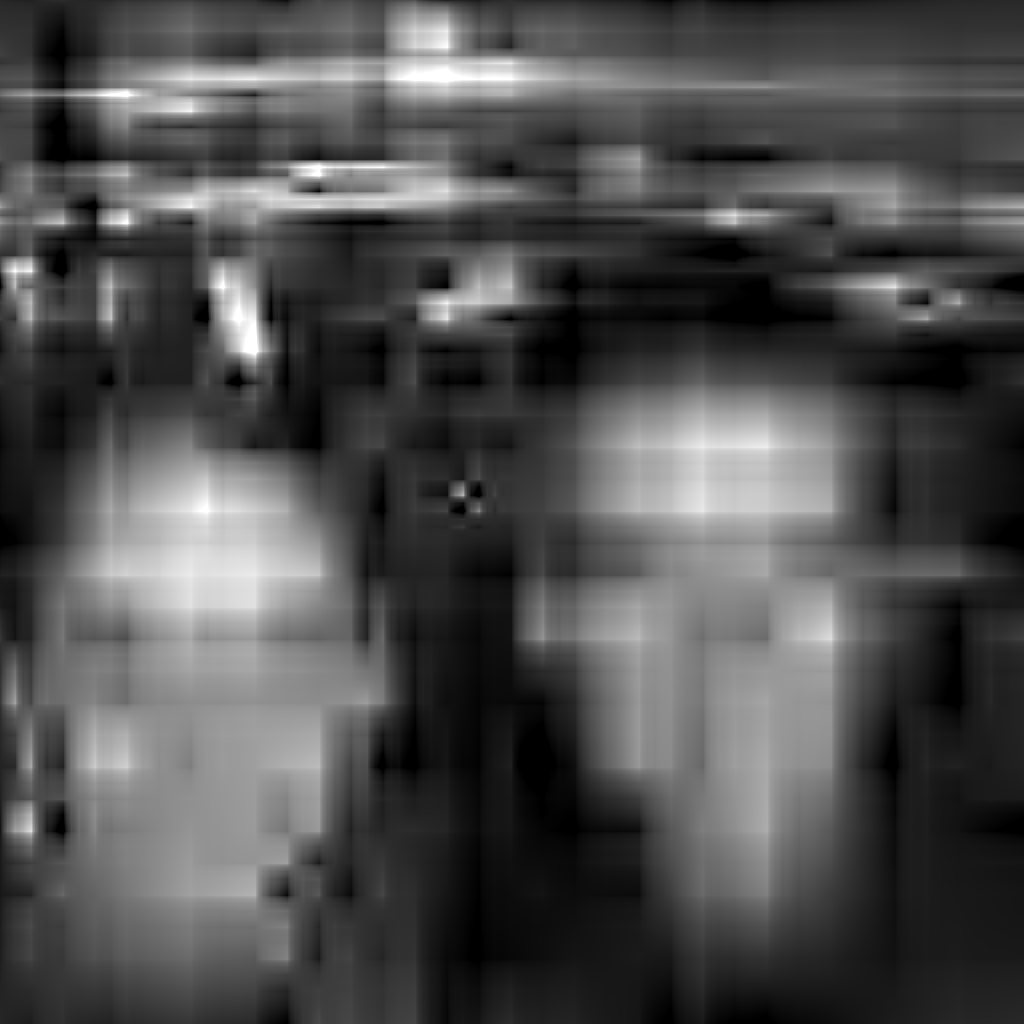
\includegraphics[width=0.3\textwidth]{parijs.png}
	\caption{My girlfriend and I in Paris. Still romantic with only 200 coefficients.}
\end{figure}
